\documentclass[margin = 1mm]{standalone}
\usepackage{scigeneral}
\usepackage{mlmodern}

\begin{document}
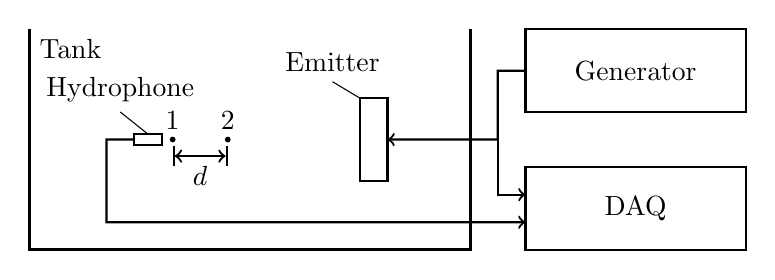
\begin{tikzpicture}[thick, scale = 0.7]
    \draw [very thick] (0, 4) -- (0,0) -- (8,0) -- ++(0,4);

    % hydrophone
    \draw (1.9,1.9) rectangle ++(0.5,0.2);

    % emitter
    \draw (6,1.25) rectangle ++(.5, 1.5);

    \fill (2.6,2) circle [radius = 1.5pt] node [above] {1};
    \fill (3.6,2) circle [radius = 1.5pt] node [above] {2};
    \draw [|<->|] (2.6, 1.7) -- ++(1, 0) node [below, pos = 0.5] {$d$};

    % generator
    \draw (9, 2.5) rectangle ++ (4, 1.5) node [pos = 0.5] {Generator};
    % DAQ
    \draw (9, 0) rectangle ++ (4, 1.5) node [pos = 0.5] {DAQ};

    % connection from the hydrophone to the DAQ
    \draw [->] (1.9, 2) -- ++(-0.5, 0) -- ++(0, -1.5) -- (9, .5);

    % connection from the Generator to the emitter
    \draw [->] (9, 3.25) -- ++(-0.5,0) -- (8.5,2) -- (6.5,2);

    % connection from the Generator to the DAQ
    \draw [->] (8.5,2) -- (8.5, 1) -- (9,1);

    % annotations
    \draw (0, 4) node [anchor = north west] {Tank};
    \draw [thin] (2.15, 2.1) -- ++(-0.5,0.4) node [anchor = south] {Hydrophone};
    \draw [thin] (6,2.75) -- ++(-.5, 0.3) node [anchor = south] {Emitter};
\end{tikzpicture}
\end{document}
